\documentclass{article}
% http://users.stat.umn.edu/~geyer/Sweave/foo.Rnw

\usepackage{amsmath}
\usepackage{amscd}
\usepackage[tableposition=top]{caption}
\usepackage{ifthen}
\usepackage[utf8]{inputenc}

\usepackage{Sweave}
\begin{document}

\title{An Sweave Demo}
\author{Charles J. Geyer}
\maketitle

This is a demo for using the \verb@Sweave@ command in R.  To
get started make a regular \LaTeX\ file (like this one) but
give it the suffix \verb@.Rnw@ instead of \verb@.tex@ and then
turn it into a \LaTeX\ file (\verb@foo.tex@) with the (unix) command
\begin{verbatim}
R CMD Sweave foo.Rnw
\end{verbatim}
So you can do
\begin{verbatim}
latex foo
xdvi foo
\end{verbatim}
and so forth.

So now we have a more complicated file chain
$$
\begin{CD}
   \texttt{foo.Rnw}
   @>\texttt{Sweave}>>
   \texttt{foo.tex}
   @>\texttt{latex}>>
   \texttt{foo.dvi}
   @>\texttt{xdvi}>>
   \text{view of document}
\end{CD}
$$
and what have we accomplished other than making it twice as annoying
to the WYSIWYG crowd (having to run both \verb@Sweave@ and \verb@latex@
to get anything that looks like the document)?

Well, we can now include R in our document.  Here's a simple example
\begin{Schunk}
\begin{Sinput}
> 2 + 2
\end{Sinput}
\begin{Soutput}
[1] 4
\end{Soutput}
\end{Schunk}
What I actually typed in \verb@foo.Rnw@ was
\begin{tabbing}
\verb@<<two>>=@ \\
\verb@2 + 2@ \\
\verb+@+ \\
\end{tabbing}
This is not \LaTeX.  It is a ``code chunk'' to be processed by \verb@Sweave@.
When \verb@Sweave@ hits such a thing, it processes it, runs R to get the
results, and stuffs (by default) the output in the \LaTeX\ file it is
creating.  The \LaTeX\ between code chunks is copied verbatim (except
for \verb@Sexpr@, about which see below).  Hence to create a Rnw document
you just write plain old \LaTeX\ interspersed with ``code chunks'' which
are plain old R.

\pagebreak[3]
Plots get a little more complicated.  First we make something to plot
(simulate regression data).
\begin{Schunk}
\begin{Sinput}
> n <- 50
> x <- seq(1, n)
> a.true <- 3
> b.true <- 1.5
> y.true <- a.true + b.true * x
> s.true <- 17.3
> y <- y.true + s.true * rnorm(n)
> out1 <- lm(y ~ x)
> summary(out1)
\end{Sinput}
\begin{Soutput}
Call:
lm(formula = y ~ x)

Residuals:
    Min      1Q  Median      3Q     Max 
-36.123  -9.321   0.987  10.352  30.110 

Coefficients:
            Estimate Std. Error t value Pr(>|t|)    
(Intercept)  -2.0799     4.3823  -0.475    0.637    
x             1.6317     0.1496  10.909 1.36e-14 ***
---
Signif. codes:  0 ‘***’ 0.001 ‘**’ 0.01 ‘*’ 0.05 ‘.’ 0.1 ‘ ’ 1

Residual standard error: 15.26 on 48 degrees of freedom
Multiple R-squared:  0.7126,	Adjusted R-squared:  0.7066 
F-statistic:   119 on 1 and 48 DF,  p-value: 1.358e-14
\end{Soutput}
\end{Schunk}
(for once we won't show the code chunk itself, look at \verb@foo.Rnw@
if you want to see what the actual code chunk was).

Figure~\ref{fig:one} (p.~\pageref{fig:one})
is produced by the following code
\begin{Schunk}
\begin{Sinput}
> plot(x, y)
> abline(out1)
\end{Sinput}
\end{Schunk}
\begin{figure}
\begin{center}
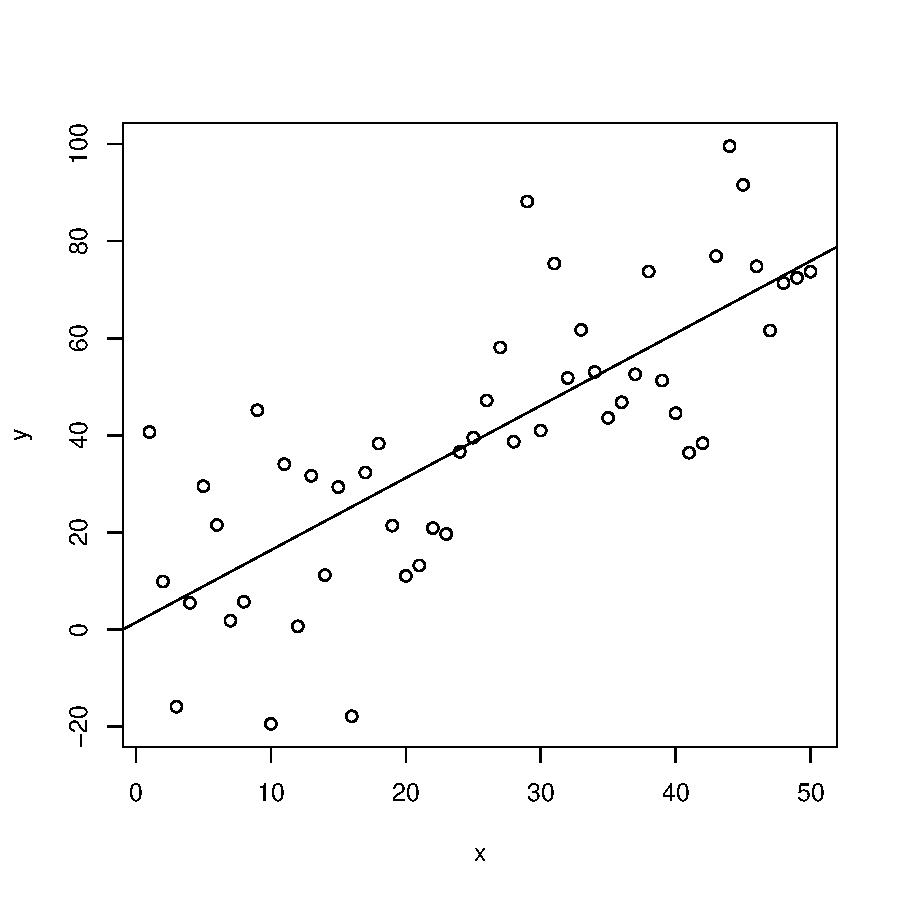
\includegraphics{foo-fig1}
\end{center}
\caption{Scatter Plot with Regression Line}
\label{fig:one}
\end{figure}
Note that \verb@x@, \verb@y@, and \verb@out1@ are remembered from
the preceding code chunk.  We don't have to regenerate them.
All code chunks are part of one R ``session''.

Now this was a little tricky.  We did this with two code chunks,
one visible and one invisible.  First we did
\begin{tabbing}
\verb@<<label=fig1plot,include=FALSE>>=@ \\
\verb@plot(x, y)@ \\
\verb@abline(out1)@ \\
\verb+@+
\end{tabbing}
where the \verb@include=FALSE@ indicates that the output (text and graphics)
should not go here (they will be some place else) and the \verb@label=fig1plot@
gives the code chunk a name (to be used later).  And ``later'' is almost
immediate.  Next we did
\begin{tabbing}
\verb@\begin{figure}@ \\
\verb@\begin{center}@ \\
\verb@<<label=fig1,fig=TRUE,echo=FALSE>>=@ \\
\verb@<<fig1plot>>@ \\
\verb+@+ \\
\verb@\end{center}@ \\
\verb@\caption{Scatter Plot with Regression Line}@ \\
\verb@\label{fig:one}@ \\
\verb@\end{figure}@
\end{tabbing}
In this code chunk the \verb@fig=TRUE@ indicates that the chunk
generates a figure.  \verb@Sweave@ automagically makes both EPS and PDF
files for the figure and automagically generates an
appropriate \LaTeX\ \verb@\includegraphics@ command
to include the plot in the \verb@figure@ environment.
The \verb@echo=FALSE@ in the code chunk means just what it says
(we've already seen the code---it was produced by the preceding chunk---and
we don't want to see it again, especially not in our figure).
The \verb@<<fig1plot>>@ is an example of ``code chunk reuse''.
It means that we reuse the code of the code chunk named \verb@fig1plot@.
It is important that we observe the DRY/SPOT rule (\emph{don't repeat yourself}
or \emph{single point of truth}) and only have one bit of code for generating
the plot.  What the reader sees is guaranteed to be the code that made the
plot.  If we had used cut-and-paste, just repeating the code, the duplicated
code might get out of sync after edits.
The rest of this should be recognizable to anyone who has ever
done a \LaTeX\ figure.

So making a figure is a bit more complicated in some ways but much simpler
in others.  Note the following virtues
\begin{itemize}
\item The figure is guaranteed to be the one described by the text
(at least by the R in the text).
\item No messing around with sizing or rotations.  It just works!
\end{itemize}

\begin{figure}
\begin{center}
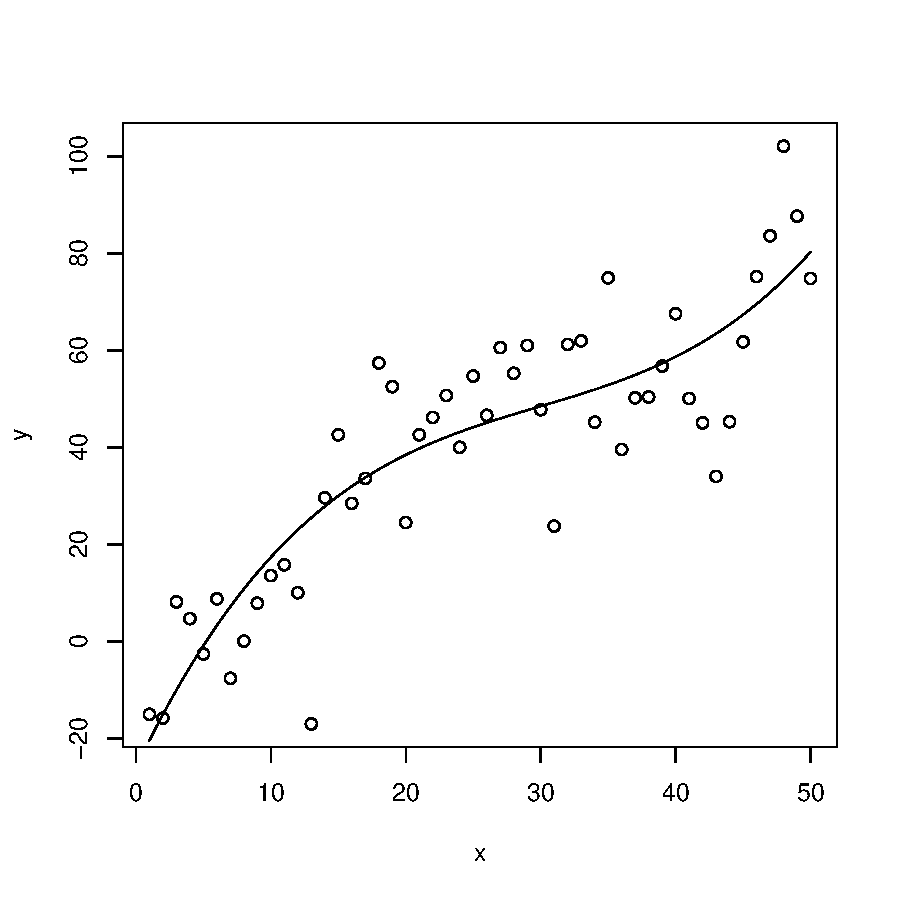
\includegraphics{foo-fig2}
\end{center}
\caption{Scatter Plot with Cubic Regression Curve}
\label{fig:two}
\end{figure}
Note that if you don't care to show the R code to make the figure,
it is simpler still.  Figure~\ref{fig:two} (p.~\pageref{fig:two})
shows another plot.
What I actually typed in \verb@foo.Rnw@ was
\begin{tabbing}
\verb@\begin{figure}@ \\
\verb@\begin{center}@ \\
\verb@<<label=fig2,fig=TRUE,echo=FALSE>>=@ \\
\verb@out3 <- lm(y ~ x + I(x^2) + I(x^3))@ \\
\verb@plot(x, y)@ \\
\verb@curve(predict(out3, newdata=data.frame(x=x)), add = TRUE)@ \\
\verb+@+ \\
\verb@\end{center}@ \\
\verb@\caption{Scatter Plot with Cubic Regression Curve}@ \\
\verb@\label{fig:two}@ \\
\verb@\end{figure}@
\end{tabbing}
Now we just included the code for the plot in the figure
(with \verb@echo=FALSE@ so it doesn't show).

Also note that every time we rerun \verb@Sweave@ Figures~\ref{fig:one}
and~\ref{fig:two} change, the latter conspicuously (because the simulated
data are random).  Everything
just works.  This should tell you the main virtue of Sweave.
It's always correct.  There is never a problem with stale
cut-and-paste.

Simple numbers can be plugged into the text with the \verb@\Sexpr@
command, for example, the quadratic and cubic regression coefficients
in the preceding regression were
$\beta_2 = -0.1677$
and
$\beta_3 = 0.0019$.
Just magic!
What I actually typed in \verb@foo.Rnw@ was
\begin{tabbing}
\verb@in the preceding regression@ \\
\verb@were $\beta_2 = \Se@\verb@xpr{round(out3$coef[3], 4)}$@ \\
\verb@and $\beta_3 = \Se@\verb@xpr{round(out3$coef[4], 4)}$.@
\end{tabbing}

The \verb@xtable@ command is used to make tables.  (The following
is the \verb@Sweave@ of another code chunk that we don't explicitly
show.  Look at \verb@foo.Rnw@ for details.)
\begin{Schunk}
\begin{Sinput}
> out2 <- lm(y ~ x + I(x^2))
> foo <- anova(out1, out2, out3)
> foo
\end{Sinput}
\begin{Soutput}
Analysis of Variance Table

Model 1: y ~ x
Model 2: y ~ x + I(x^2)
Model 3: y ~ x + I(x^2) + I(x^3)
  Res.Df     RSS Df Sum of Sq      F  Pr(>F)  
1     48 11180.7                              
2     47 10144.5  1   1036.15 5.1971 0.02731 *
3     46  9171.1  1    973.43 4.8825 0.03215 *
---
Signif. codes:  0 ‘***’ 0.001 ‘**’ 0.01 ‘*’ 0.05 ‘.’ 0.1 ‘ ’ 1
\end{Soutput}
\begin{Sinput}
> class(foo)
\end{Sinput}
\begin{Soutput}
[1] "anova"      "data.frame"
\end{Soutput}
\begin{Sinput}
> dim(foo)
\end{Sinput}
\begin{Soutput}
[1] 3 6
\end{Soutput}
\begin{Sinput}
> foo <- as.matrix(foo)
> foo
\end{Sinput}
\begin{Soutput}
  Res.Df       RSS Df Sum of Sq        F     Pr(>F)
1     48 11180.659 NA        NA       NA         NA
2     47 10144.506  1  1036.153 5.197103 0.02730910
3     46  9171.075  1   973.431 4.882505 0.03214702
\end{Soutput}
\end{Schunk}
So now we are ready to turn the matrix \verb@foo@
into Table~\ref{tab:one}
% latex table generated in R 3.0.2 by xtable 1.7-3 package
% Sun May 25 01:06:37 2014
\begin{table}[tbp]
\centering
\caption{ANOVA Table} 
\label{tab:one}
\begin{tabular}{rrrrrrr}
  \hline
 & Res.Df & RSS & Df & Sum of Sq & F & Pr($>$F) \\ 
  \hline
1 & 48 & 11180.66 &  &  &  &  \\ 
  2 & 47 & 10144.51 & 1 & 1036.15 & 5.197 & 0.027 \\ 
  3 & 46 & 9171.08 & 1 & 973.43 & 4.883 & 0.032 \\ 
   \hline
\end{tabular}
\end{table}using the R chunk
\begin{tabbing}
\verb@<<label=tab1,echo=FALSE,results=tex>>=@ \\
\verb@library(xtable)@ \\
\verb@print(xtable(foo, caption = "ANOVA Table", label = "tab:one",@ \\
\verb@    digits = c(0, 0, 2, 0, 2, 3, 3)), table.placement = "tbp",@ \\
\verb@    caption.placement = "top")@ \\
\verb+@+
\end{tabbing}
(note the difference between arguments to the \verb@xtable@ function
and to the \verb@xtable@ method of the \verb@print@ function).

To summarize, \verb@Sweave@ is terrific, so important that soon
we'll not be able to get along without it.  It's virtues are
\begin{itemize}
\item The numbers and graphics you report are actually what they
are claimed to be.
\item Your analysis is reproducible.  Even years later, when you've
completely forgotten what you did, the whole write-up, every single
number or pixel in a plot is reproducible.
\item Your analysis actually works---at least in this particular instance.
The code you show actually executes without error.
\item Toward the end of your work, with the write-up almost done you
discover an error.  Months of rework to do?  No!  Just fix the error
and rerun \verb@Sweave@ and \verb@latex@.  One single problem like
this and you will have all the time invested in \verb@Sweave@ repaid.
\item This methodology provides discipline.
There's nothing that will make you clean up your code like
the prospect of actually revealing it to the world.
\end{itemize}

Whether we're talking about homework, a consulting report, a textbook,
or a research paper.  If they involve computing and statistics,
this is the way to do it.

\end{document}
